\chapter{Realisierung des Source-To-Source Compilers}
\label{chap:Realisierung}
Gestützt auf das grundsätzliche Wissen über Compiler, die herausgearbeiteten Unterscheidungen von  Xamarin.Forms und Flutter sowie die Differenzen der verwendeten Programmiersprachen  \Csharp und Dart, wird in diesem Kapitel die Realisierung des Source-To-Source Compilers beschrieben.  Es bietet sich die \ac{ide} (deutsch Entwicklungsumgebung) Visual Studio 2019 von Microsoft an,  um das Projekt mit Roslyn Integration zu implementieren,  denn auf dieser Plattform stehen Erweiterungen für Roslyn zur Verfügung.
Die zu entwickelnde Projektmappe,  besteht also aus dem Source to Source Compiler mit Rosyln Integration, der grafischen Benutzeroberfläche und einer Xamarin.Forms
Anwendung als Testobjekt,  wobei letztere jedoch erst im nächsten Kapitel thematisiert wird.


\section{Programmablauf}
Mithilfe des Roslyn Compilers kann der Source-To-Source Compiler Auswertungen zu den in der Xamarin.Forms App referenzierten Quelltextdateien durchführen.  Somit ist es
möglich eine Auflistung aller verfügbaren \Csharp - Dateien aus einem Projekt zu extrahieren.  XAML -Dateien werden nicht von Roslyn behandelt.  Dies gelingt jedoch über den Umweg der Codebehind-Dateien mit Endung .XAML.CS,  die ein Laden über das Dateisystem ermöglichen. 

Nachdem der Source-To-Source Compiler alle Quelltext- und Ansichtsdateien übersetzt hat,  müssen die in Kapitel 4 beschriebenen Metadaten überführt werden.  Anschließend kann der Quelltext optimiert und der Übersetzungsvorgang abgeschlossen werden.  Folgend kann nun zur Visualisierung des Übersetzungsvorganges ein \ac{uml}  Aktivitätsdiagramm angelegt werden, wie es in Abbildung \ref{fig:umlablauf} dargestellt ist.

\newpage
\begin{figure}[!ht]
 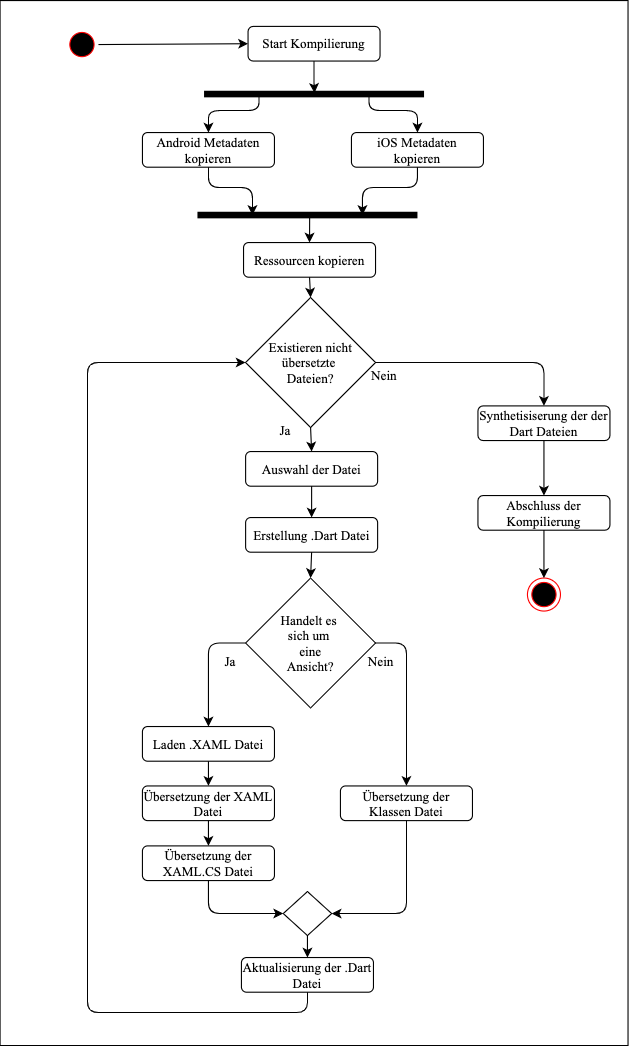
\includegraphics[width=\textwidth,keepaspectratio]{Images/Implementation/Ablauf.png}
 \caption{Aktivitätsdigramm}
 \label{fig:umlablauf}
\end{figure}

Das dargestellte \ac{uml}-Diagramm befindet sich aufgrund der Komplexität des Compilers auf einer hohen Abstraktionsebene. In den folgenden Abschnitten werden die einzelnen Aspekte der Kompilierung noch näher betrachtet.


\section{Metadaten}
Wie das UML Diagramm veranschaulicht können die Metadaten von Android und iOS parallel in die Flutter Anwendung kopiert werden.  Da die Metadaten
plattformspezifische Eigenschaften der mobilen Anwendungen sind, wird im nächsten Abschnitt auf die entsprechenden Details der beiden Betriebssysteme eingegangen.


\subsection{Android Metadaten}
Zu den Android spezifischen Metadaten gehören die sogenannten Launcher Icons, die den Anwendern als App-Icon angezeigt werden. Xamarin.Android speichert diese grafischen Symbol in Ordnern, die die unterschiedlichen Pixeldichten der Android-Geräte unterstützen und in denen unter Umständen auch andere Bilder gespeichert sind.  Innerhalb von Xamarin.Forms wird das ausgewählte Icon über die Klasse MainActivity.cs definiert, wie dies in Quelltext \ref{lst:IconName} dargestellt ist. 

\lstinputlisting[label={lst:IconName},caption={Xamarin.Forms Android Launcher-Icon Name}, language=csh]{SourceCode/IconName.cs}

Nach der Extraktion des Namens können nun die entsprechenden Bilder kopiert werden.  In der durch die Flutter SDK erzeugten App liegen bereits Bildplatzhalter zum Austausch bereit.

Der eindeutige Identifizierer,  PackageID,  zählt ebenfalls zu den Metadaten und dient zur eindeutigen Erkennung der Anwendungen auf dem mobilen Gerät und im GooglePlay Store.  Die Information über die ID kann in Xamarin.Forms aus der AndroidManifest.XML Datei ausgelesen  werden, und muss aber in Flutter sowohl in 3 Manifest Dateien als auch in die build.gradle geschrieben werden.Das Plugin,  change\_app\_package\_name , nimmt alle notwendigen Änderungen vor. Es muss als Abhängigkeit zum Projekt hinzugefügt und anschließend über die Kommandozeile ausgeführt werden. 

Der Anwendungsname wird, wie die PackageID, aus dem AppManifest extrahiert und in Flutter allerdings auch nur in eine Manifest Datei im Verzeichnis Project/app/src/main’ geschrieben.  Auch die Berechtigungen, die während der Laufzeit der Anwendung, beantragt werden befinden sich innerhalb des AppManifests und können auch kopiert werden.

\subsection{iOS Metadaten}
Xamarin.iOS verwaltet Metadaten die für die Übersetzung notwendig sind ebenfalls in einer Datei im Projektverzeichnis mit dem Namen Info.plist.  In Flutter Apps gibt es eine entsprechende Datei,  jedoch werden die Inhalte,  beispielsweise die Bildnummer und der Identifizierer,  aus Variablen geladen.  Damit nach der Kompilierung keine Besonderheiten in der Administration der Flutter App entstehen,  soll dieses Schema beibehalten werden.  Die AppFrameworkInfoPlist stellt die Quelle aller Werte,  die als Variablen in die Info.plist, geladen werden müssen dar.   Daher werden die entsprechenden Einträge aus der Info.Plist von Xamarin extrahiert und jeweils in die entsprechenden Info.Plist Dateien von Flutter kopiert.  Eine entsprechende Gegenüberstellung, welcher Wert in welche Datei überführt werden muss,  wird in Tabelle \ref{tab:InfoPlist} dargestellt. 


\begin{table}[!ht]
  \begin{tabularx}{\linewidth}{X| X| X}
  \textbf{Schlüssel}  &  \textbf{Info.plist} & \textbf{AppFrameworkInfo.plist} \\
\hline
  DevelopmentRegion  		&  					& 		\checkmark	 \\
  ShortVersionString  		&  					& 		\checkmark	 \\
  Version  							&  					& 		\checkmark	 \\
  MinimumOSVersion  		&  					& 		\checkmark	 \\
  
  InterfaceOrientations  		& \checkmark  	&		 					\\
  BundleSignature  			&  \checkmark 	& 							\\
   BundleName  					&  \checkmark 	& 		 					\\
\end{tabularx}
\caption{Plist Dateien in Flutter }
 \label{tab:InfoPlist}
\end{table}
Die Tabelle weist nicht alle in iOS bekannten Schlüssel auf,  alle fehlenden werden in Flutter in der Datei Info.Plist ergänzt.

Für das Anwendungsoicon kann das Verzeichnis Assets.xcassets aus dem Stammverzeichnis der Xamarin.Forms iOS App in das Verzeichnis ios/flutter/Runner, das alle notwendigen Bilder enthält,  kopiert werden. 

\section{Ressourcen}

Neben diesen Metadaten müssen auch die Ressourcen der mobilen Anwendung kopiert werden. 
Dazu gehören die innerhalb der App angezeigten Bilder, die bei Xamarin.Forms
üblicherweise innerhalb der plattformspezifischen Anwendungen abgelegt sind.
Von dort aus kopiert der Compiler die Bilder aus dem iOS Projekt in das Flutter Projekt zur spätere Verwendung.  Da für Bilder im Flutter Framework keine plattformspezifische Unterscheidung vorgesehen ist,  werden ausschließlich die von iOS entnommen. Eine Entscheidung zugunsten der iOS Alternativen wurde  entschieden,  da sich die Konzepte von Xamarin.iOS und Flutter im Bezug auf Bilderressourcen ähneln und eine automatisierte Überführung möglich ist.  Android spezifische Varianten werden während der Übersetzung also nicht berücksichtigt.   
Zur Speicherung und Darstellung höher aufgelöster Bilder existieren zwei Unterordner mit den Namen 2.0x und 3.0x im Verzeichnis Assets.  Ressourcen werden je nach Skalierungsoption @2x oder @3x in den Verzeichnissen abgelegt. Dateien ohne diese Skalierungsoption werden im Ordner Asset gespeichert.
Neben dem differenzierten Vorgehen bei der Kopierung ist es erforderlich die Ressourcen in der pubspec.yaml zu referenzieren.  Ein Ausschnitt aus der Pubspec.yaml der das Einbinden von Bildern demonstriert wird in Quelltext  \ref{lst:RefImage} dargestellt.

\lstinputlisting[label={lst:RefImage},caption={Referenzierung von Bildern in der Pubspec.yaml}, language=Dart]{SourceCode/FlutterPubspecImage.pub} 


Benutzerdefinierte Schriftsätze werden ebenfalls aus dem iOS Verzeichnis kopiert und anschließend in der pubspec.yaml Datei hinzugefügt.  Hier gilt,  analog zu den Bildern,  das die kompilierte Flutter Anwendung ausschließlich die Schrift der iOS App verwendet und Android spezifische Schriftsätze verloren gehen.

Eine weitere Ressource bilden die Startbildschirme der verschiedenen Plattformen,  die während des Ladens der App angezeigt werden und für eine Veröffentlichung im Appstore verpflichtend sind.  Durch ihren simplen Aufbau wird keine zusätzliche Ladezeit generiert.  Startbildschirme werden über plattformspezifischen Quelltext realisiert.   Der Compiler verarbeitet ausschließlich einzelne Bilder die während des Ladens der mobilen Anwendung angezeigt werden.  Das beschriebene Vorgehen ist von Xamarin.Forms nicht vorgesehen, daher kann bei der Übersetzung von keinem Bild im entsprechenden Format ausgegangen werden. Alternativ wird bei der Erstellung des Flutter Ladebildschirms auf das LauncherIcon der jeweiligen Plattformen zurückgegriffen.  

\section{Übersetzung von Klassenstrukturen}

Die Übersetzung von \Csharp zu Dart ist ein essentieller Bestandteil des Compilers.  Dafür wird zuerst die Visual Studio Projektmappe geladen.  Da in dieser Arbeit kein plattformspezifischer Quelltext betrachtet wird,  sind die entsprechende  Projekte ausschließlich für das Kopieren der Metadaten und Ressourcen notwendig.  Anschließend kann ausschließlich das Projekt betrachtet werden, welches den plattformunabhängigen Quelltext beinhaltet.  Dabei wird für alle Klassen der in  \ref{lst:CsharpFrontend} dargestellte Quelltext ausgeführt. 
\lstinputlisting[label={lst:CsharpFrontend},caption={C\# Compiler Frontend}, language=csh]{SourceCode/CompilerFrontEnd.cs}
Für die Übersetzung von einer Programmiersprache zu einer anderen ist es notwendig,  alle Knoten und Token innerhalb eines Syntaxbaums in der richtigen Reihenfolge zu betrachten.  Die abstrakte Klasse \glq CSharpSyntaxWalker\grq{} erlaubt es einen eigenen \glq Syntax-Walker\grq{} zu konstruieren,  der alle Knoten und Token analysieren kann.  Dafür kann von \glq CSharpSyntaxWalker\grq{} geerbt werden und anschließend die \glq Visit()\grq{} Methode überschreiben werden.  \footcite[Vgl.][Abgerufen am \today]{Varty2014}  Der Quelltext visualisiert die Erstellung eines \glq FlutterTranspilerVisitors\grq{} mithilfe des vorher ermittelten semantischen Models.  Anschließend wird der ausgelesene Wurzelknoten des Syntaxbaumes als Parameter der \glq Run()\grq{} Methode übergeben, welches den \glq Visitor\grq{} startet.  


Diese Schritte beschreiben das Compiler-Frontend,  anschließend kann der Dart Quelltext konstruiert werden.  Dafür werden die einzelnen Knoten des Baumes je nach ihrem Typen zu entsprechenden Dart Synonymen umgewandelt.  Dafür werden die einzelnen Methoden des \glq CSharpSyntaxVisitor\grq{} überschrieben.  So zeigt Quelltext \ref{lst:PropertyDeclaration} die Umwandlung von Eigenschaftsdeklarationen.
\newpage
\lstinputlisting[label={lst:PropertyDeclaration},caption={Compilierung von Eigenschaftsdeklarationen}, language=csh]{SourceCode/Modifizierer.cs}

Der Quelltextausschnitt veranschaulicht die generelle Arbeitsweise des Compilers,  bei der die einzelnen Zeichen und Zeilen des Dart-Textdokumentes generiert und anschließend in gespeichert werden.  So hangelt sich der Compiler durch das Dokument und übersetzt den Quelltext Schritt für Schritt, wobei die Reihenfolge in denen der 
Typ, der Modifizierer und Name der Eigenschaft in die Dart Datei geschrieben wird essentiell ist.
n.  So wird in den Quelltextzeilen 6 bis 8 zuerst der Typ der Eigenschaft ausgegeben gefolgt von dem optionalen Modifizierer und dem Namen.   Anschließend wird optional ein Wert gesetzt und die Reihe mit einem Semikolon abgeschlossen.  Die Methode für die Generierung des Dart Modifizierers wird in Quelltext \ref{lst:DartModifier} dargestellt.

\lstinputlisting[label={lst:DartModifier},caption={Austausch von C\# Modifizierern}, language=csh]{SourceCode/Modifier.cs}


Wie bereits in Kapitel 5 beschrieben sind die auszugebenden Typen der Programmiersprachen nicht identisch und müssen daher entsprechend angepasst werden.  Zur  Veranschaulichung wird die realisierte Methode in Quelltext {lst:DataType} dargestellt. 
\lstinputlisting[label={lst:DataType},caption={Austausch von C\# Datentypen}, language=csh]{SourceCode/Datatypes.cs}

Diese Methode gibt den Namen des jeweiligen Dart-Datentypen,  für die jeweiligen \Csharp Repräsentationen zurück.  Am Ende der Methode wird,  wenn kein passender Datentyp ermittelt werden konnte der Name des ursprünglichen Typen zurück gegeben.  Dies ist notwendig um selbst entwickelten Klassen verwenden zu können. 

%Was passiert mit .Net klassen? Fehler ausgegeben? 

Wie in Kapitel 4 beschrieben werden viele Funktionalitäten mithilfe von Erweiterungen ermöglicht.  Jedoch sind die Erweiterungen die,  wenn auch vergleichbar, von anderen
Herstellern mit unterschiedlichen Anforderungen programmiert wurden.  Daraus folgt,  dass es für Klassen und Methoden aus diesen Bibliotheken nicht zwangsläufig identischen Repräsentationen gibt.  Diese Inkompatibilität kann nicht mittels Automation gelöst werden und Bedarf daher unterschiedlich umfangreicher manueller Umwandlungen.  Ein Beispiel soll zeigen,  wie Konflikte aufgelöst werden können.  Der Compiler wird jedoch nur diesen Falle enthalten, weitere Umwandlungen von Plugins müssen im Rahmen von Erweiterungen ergänzt werden.  Als Beispiel soll der bereits in Abschnitt 3.5 eingeführte Anwendungsfalle wieder aufgegriffen werden indem ein Bild aus dem Bilderalbum des Gerätes ausgewählt wird.  So geben die Funktionen von sowohl von Xamarin.Forms als auch von Flutter jeweils ein Objekt zurück, welches das ausgewählte Bild repräsentiert.  Beide haben jedoch unterscheide,   das Flutter Objekt kann mit den Methoden readAsBytes und readAsString gelesen werden,  während das Xamarin.Forms Bild mit der Methode OpenReadAsync geladen werden kann.  Daher ist es notwendig neben der Zuordnung der Erweiterungen auch ein Mapping der Methoden vorzunehmen. Obwohl es keine Gewährleistung gibt, dass für jede Xamarin Forms eine entsprechende Flutter 
Erweiterung zur Verfügung steht, konnte bei der Implementierung des Compilers immer eine  Alternative gefunden werden.


\section{Übersetzung von Ansichten}
Die Übersetzung von Ansichten inkludiert die XAML und XAML.cs Dateien, die nach der Übersetzung von Klassenstrukturen in einer gemeinsamen Dart-Datei synthetisiert werden müssen.  Daraus folgt,  dass für beide Typen von Ursprungsdateien jeweils ein Compiler Front-End,  das die Aufgaben bis zur Zwischendarstellung übernimmt entwickelt werden muss und darauf basierend in einem gemeinsamen Compiler-Backend die Zusammenführung sowie die Code-Optimierung durchgeführt wird.  Die Abbildung  \ref{fig:ViewCompilerPhases} visualisiert den Vorgang. 

\begin{figure}[!ht]
 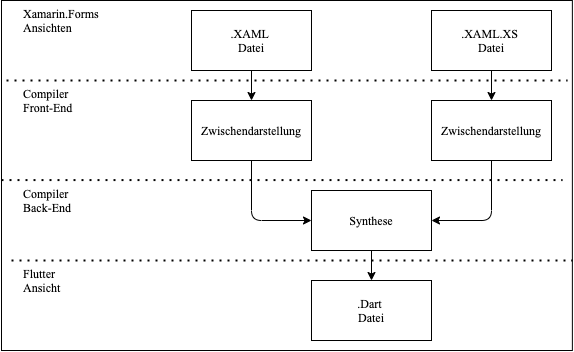
\includegraphics[width=\textwidth,keepaspectratio]{Images/Implementation/ViewCompiler.png}
 \caption{Compiler Phasen für Ansichten}
 \label{fig:ViewCompilerPhases}
\end{figure}

\subsection{Visuellen- Zwischendarstellung}

Für die visuelle Zwischendarstellung wird in einem ersten Schritt die XML Struktur
aus der XAML Datei ausgelesen und ein Syntaxbaum angelegt.  Die entsprechenden Klassen für die Darstellung des Syntaxbaumes werden in Abbildung \ref{fig:Klassendiagram} in Form eines Klassendiagramm dargestellt..

\begin{figure}[!ht]
 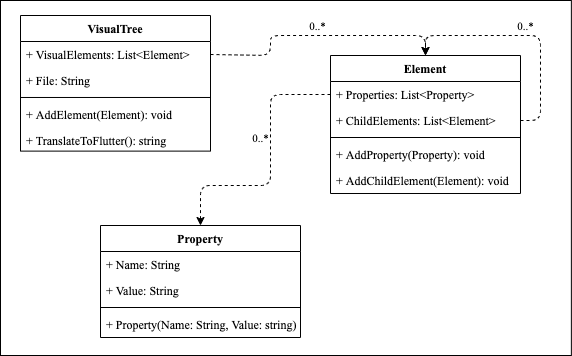
\includegraphics[width=\textwidth,keepaspectratio]{Images/Implementation/Klassendiagram.png}
 \caption{Klassendiagramm}
 \label{fig:Klassendiagram}
\end{figure}

Ein Objekt der Klasse VisualTree stellt den Layout-Baum einer speziellen XAML Datei dar.  Er beinhaltet eine Auflistung von untergeordneten Elementen, welche wiederum weitere Elemente beinhalten können um die Verschachtlung des Baumes abzubilden.  Jedes Element besitzt eine Auflistung von Eigenschaften, die Attribute der einzelnen XML Knoten beschreiben.  Dieser Baum wird anschließend,  durch die in Kapitel 4 beschriebenen Gegenüberstellungen von Flutter Widgets, in einen Flutter Widget-Baum überführt.  Dabei wird für jedes Widget der Quelltext zur Initialisierung in einem Template vorgehalten.  Alle möglichen Variablen und Eigenschaften dieser Widgets werden innerhalb dieser Vorlagen mit Platzhaltern bereitgestellt.  Dies wird in Quelltext \ref{lst:Placeholder} dargestellt.

\lstinputlisting[label={lst:Placeholder},caption={Flutter Widget mit Placeholdern} , language=Dart]{SourceCode/DartPlaceholder.dart} 

Nun erfolgt im nächsten Schritt das Extrahieren der Eigenschaften des Quellframeworks und im 
Anschluss die Eintragung des Codes in das Template.  Neben den Eigenschaften die einen Wert in XAML,  definiert haben gibt es auch noch Eigenschaften,  die über sogenannte Databindings aus den Codebehind-Daten gefüllt werden,  für deren Übersetzung neue Platzhalter mit dem Prefix Databinding in dem Template hinterlegt 
werden. In einem späteren Arbeitsschritt ist eine Bereinigung des Templates erforderlich,  denn ungenutzte Platzhalter müssen entfernt werden.



\subsection{Logische- Zwischendarstellung}

Für die Erzeugung der logischen Zwischendarstellung wird die gleiche Logik wie für die Klassenstrukturen verwendet,  da es sich bei diesen Dateien ausschließlich um \Csharp Klassen handelt.  Damit sich die Benutzeroberfläche automatisch aktualisiert müssen noch erweiterte Änderungen vorgenommen werden.
Während bei Xamarin.Forms Änderungen an Eigenschaften automatisch an die Benutzeroberfläche 
übermittelt werden, muss bei Flutter das Framework mithilfe der setState()) Methode  informiert 
werden.  Anpassungen am Quelltext können nicht während der Erstellung der Zwischendarstellung 
geschehen, denn die eigentlich dafür zuständige Codebehind Datei ist nicht darauf ausgelegt zu 
erkennen, welche Eigenschaften einen direkten Bezug zur Ansicht haben.  Daher erfolgt dieser Schritt im Compiler Backend.

\section{Synthese}

Die Synthese ist eine Teilaufgabe des Compiler Backend  und befasst sich mit der Zusammenführung der einzelnen Zwischendarstellungen.  Dafür werden die gesamten Methoden und Eigenschaften aus der logischen Darstellung in die Ansicht überführt und die Referenzierungen dort entsprechend angepasst.  Zu diesem Zeitpunkt kann ermittelt werden, welche Eigenschaften und Methoden im UI zu 
Veränderungen führen.   Quelltextstellen,  die eine Oberflächenaktualisierung auslösen sollen,  müssen folglich in einen SetState Block eingefügt werden, damit Änderungen automatisch in App angezeigt werden.

%Quelltext

In einem ersten Schritt werden die Zwischendarstellungen der Codebehind Datei und der Ansicht kombiniert.  Dafür wird die übersetzte Logik unterhalb der für den Aufbau der grafischen Benutzeroberfläche beinhaltenden Build Methode hinterlegt.  Im nächsten Schritt werden ereignisauslösende Aktivitäten, beispielsweise der Klick auf 
Schaltflächen,  mit den übersetzen Methoden verbunden und die Platzhalter entfernt. Eine Überprüfung welche Eigenschaften der Codebehind-Klassen am Front-End Änderungen durchgeführt haben, wird mittels Binding Platzhaltern vollzogen.  So müssen alle Bereiche im Quelltext, die Änderungen an Eigenschaften vornehmen zu denen es ein Binding-Placeholder gibt mit einem SetState Block umschlossen werden.

%Quelltext

Jetzt können die nicht benötigten Platzhalter entfernt werden.  Damit befindet sich der Quelltext in einem korrekten syntaktischen Zustand und kann mit Hilfe des Flutter Compilers zu einer mobilen App übersetzt und ausgeführt werden. 


\section{Grafische Benutzeroberfläche}
Die GUI ist der zentrale Berührungspunkt von Anwendern mit dem Transpiler.  Sie soll die notwendigen Eingabe-Möglichkeiten anbieten, das Ergebnis ausgeben und den Anwender auf mögliche Fehler hinweisen.  Das grafische Vorbild ist das in Kapitel 3 entworfene Mockup, siehe Abbildung 3.4.  Für die Erstellung einer entsprechenden Benutzeroberfläche stehen eine Vielzahl von Technologien mit verschiedenen Vor- und Nachteilen zur Verfügung.  Eine Webseite wäre von Vorteil, da Anwender keinen Installationsaufwand hätten und  plattformunabhängig auf den Compiler zugreifen könnten.  Allerdings ist zumindest ein gewisser Kontrollverlust über den eigenen Quelltext durch das  Hochladen auf eine Webseite nicht ausgeschlossen.  Die Bedienoberfläche dieser Arbeit soll daher eine lokale Anwendung sein, sodass kein  unberechtigter Zugriff auf den Source-Code möglich ist. Zu diesem Zwecke wird die GUI mit der Technologie \ac{wpf}  realisiert. Dabei handelt es sich um ein UI-Framework des .NET Frameworks, das für die Erstellung von Desktopanwendungen geeignet ist und mit XAML und \Csharp entwickelt wird. \footcite[Vgl.][S. 1f]{Wenger2012} 

Anwendungen die mittels WPF programmiert werden, sind nur unter Windows als Betriebssystem ausführbar.  Da der Roslyn Compiler jedoch auch nur für Windows Computer zur Verfügung steht entstehen hier keine zusätzlichen Einschränkungen. 

Die folgenden Bilder visualisieren das Aussehen der Anwendung nach einer erfolgreichen Übersetzung. 

<Screenshot Anwendung >

Wie die Ansicht visualisiert werden in der Anwendung umfangreiche Logs angezeigt,  die durchgeführten Arbeitsschritte dokumentieren.  Da dieser Compiler im Regelfall nur einmal verwendet wird um eine mobile Anwendung zu übersetzen,  gibt es  die Möglichkeit das Ergebnis der Übersetzung mit den Log-Dateien zu speichern und zu einem späteren Zeitpunkt erneut zu laden ohne den Übersetzungsvorgang erneut durchführen zu müssen.

Da sowohl die grafische Benutzeroberfläche als auch der Source-To-Source Compiler mit .Net Technologien realisiert wurden lassen sie sich einfach miteinander kombinieren.  Dafür wird der Compiler als Abhängigkeit in das Projekt der grafischen Benutzeroberfläche geladen.  Dies ist Notwendig,  damit die grafische Benutzeroberfläche den Übersetzungsvorgang starten kann. 

\section{Zusammenfassung}
Während der Realisierung des Compilers wurden Entscheidungen getroffen, die für eine nicht vollständig identische Übersetzung verantwortlich sind.  So wurden Bilder ausschließlich aus IOS Projekten entnommen und die Startbildschirme der Xamarin Forms Anwendungen auf eine Bilddarstellung reduziert.
